%Based on the code of Yiannis Lazarides
%http://tex.stackexchange.com/questions/42602/software-requirements-specification-with-latex
%http://tex.stackexchange.com/users/963/yiannis-lazarides
%Also based on the template of Karl E. Wiegers
%http://www.se.rit.edu/~emad/teaching/slides/srs_template_sep14.pdf
%http://karlwiegers.com
\documentclass{scrreprt}
\usepackage{listings}
\usepackage{underscore}
\usepackage[margin=3.0cm]{geometry}
\usepackage{enumitem}
\usepackage{graphicx}
\usepackage[bookmarks=true]{hyperref}
\usepackage[english, spanish]{babel}
\usepackage[utf8]{inputenc}
\usepackage{float}
\usepackage{xcolor}
\usepackage{fancyhdr}
\usepackage[export]{adjustbox}

\hypersetup{
    bookmarks=false,        % show bookmarks bar?
    pdftitle={Especificación de Requerimientos de Software},    % title
    pdfauthor={},           % author
    pdfsubject={},          % subject of the document
    pdfkeywords={},         % list of keywords
    colorlinks=true,        % false: boxed links; true: colored links
    linkcolor=blue,         % color of internal links
    citecolor=black,        % color of links to bibliography
    filecolor=black,        % color of file links
    urlcolor=purple,        % color of external links
    linktoc=page            % only page is linked
}

\def\myversion{1.0}
\date{}
\usepackage{hyperref}
\usepackage{etoolbox}

%%%%%%%%%%%
% Configurar estilo de header y footer
\fancypagestyle{plain}{
  \fancyhf{}
  \lfoot{
\includegraphics[scale=0.08,valign=c]{images/space_logo.png}}
  \rfoot{Pág. \thepage}
}

\pagestyle{fancy}
\fancyhf{}
\lfoot{
\includegraphics[scale=0.08,valign=c]{images/space_logo.png}}
\rfoot{Pág. \thepage}

\renewcommand{\headrulewidth}{0pt} % linea de header invisible
\renewcommand{\footrulewidth}{0.4pt} % linea de footer delgada

%%%%%%%%%%

\begin{document}

\begin{flushright}
	\rule{16cm}{0.2cm}\vskip1cm
    \begin{bfseries}
        \Huge{ESPECIFICACIÓN DE ARQUITECTURA DEL SISTEMA}\\
        \vspace{0.5cm}
        para\\
        \vspace{0.5cm}
        Sistema de preprocesamiento y segmentación de células\\
        \vspace{1.0cm}
        \LARGE{Modelo 4 + 1}\\
        \vspace{1.0cm}
        Preparado por:\\ \vspace{0.5cm}
        	José Alvarado Chaves, 201129079\\
            Reggie Barker Guillén, 2014050578\\
            Joel Barrantes Garro, 2013120962\\
            Joel Schuster Valverde, 2014096796\\                        
        \vspace{1.5cm}
        Instituto Tecnológico de Costa Rica\\
        \vspace{1.5cm}
        \today\\
    \end{bfseries}
\end{flushright}


\tableofcontents


\chapter{El Modelo 4 + 1}

El modelo 4 + 1 es un modelo diseñado por Philippe Kruchten para describir la arquitectura de sistemas software, basados en el uso de múltiples vistas concurrentes. Las vistas suelen describir el sistema desde la perspectiva de los diferentes interesados, tales como usuarios finales, desarrolladores o directores de proyecto. Las cuatro vistas del modelo son: vista lógica, vista de despliegue, vista de proceso y vista física. Además, una selección de casos de uso o escenarios suele utilizarse para ilustrar la arquitectura sirviendo como una vista más.\\

\begin{figure}[H]
	\centering
    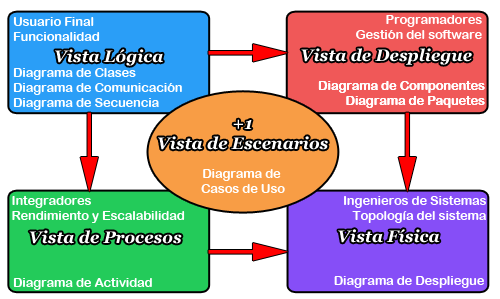
\includegraphics[width=0.8\linewidth]{images/Kruchten.png}
    \caption{Ilustración del modelo 4 + 1 de Kruchten}\label{Kruchten}
\end{figure}

\chapter{Vista lógica}

La vista lógica está enfocada en describir la estructura y funcionalidad del sistema. Los diagramas UML que se suelen utilizar para representar esta vista son los diagramas de clase, de estado, de comunicación y de secuencia.\\

\section{Diagrama de clases}

\begin{figure}[H]
	\centering
    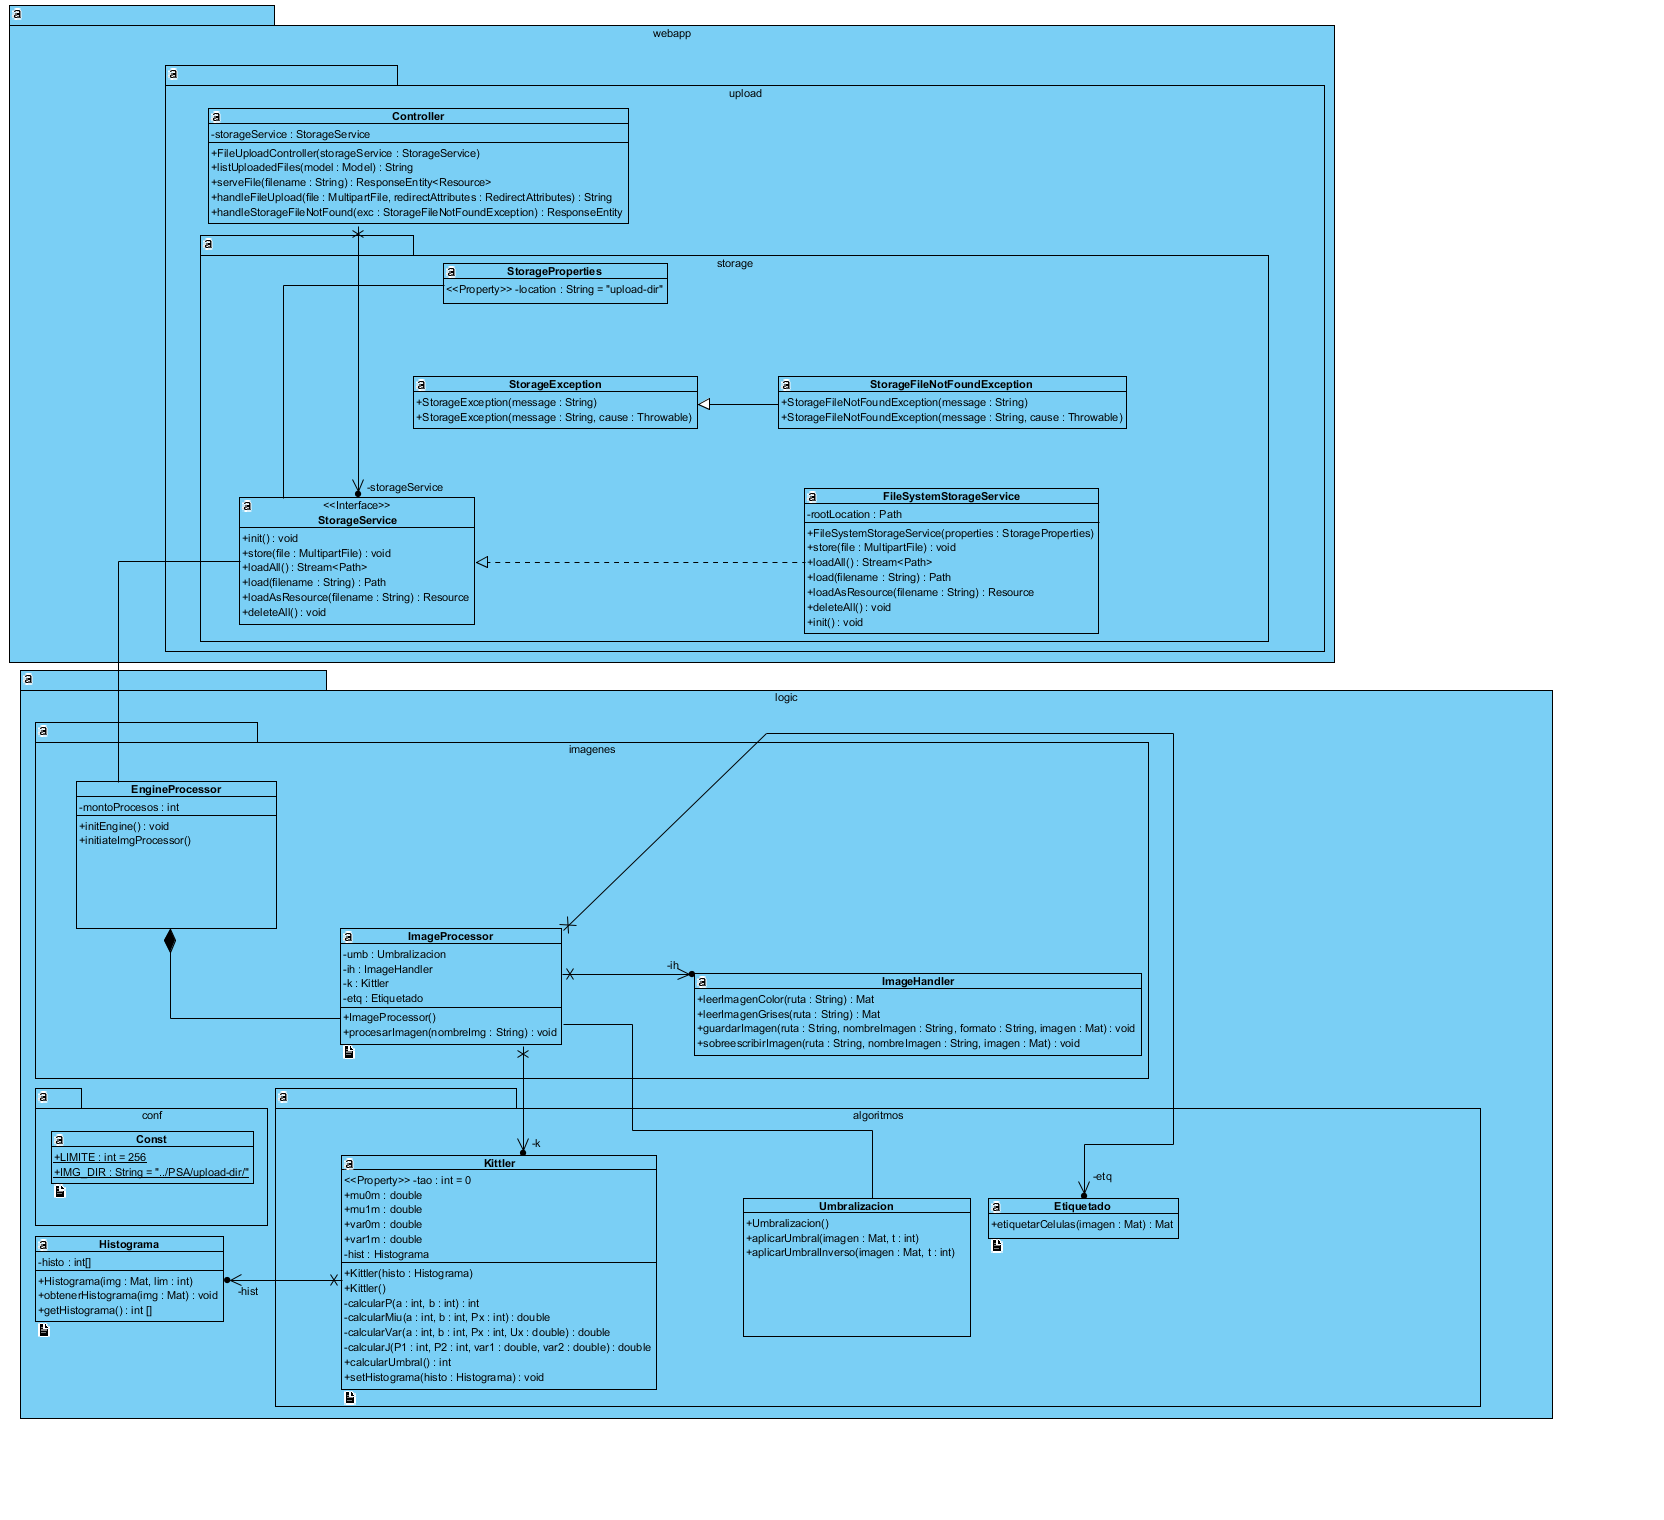
\includegraphics[width=1\linewidth]{images/diagramaClases.png}
    \caption{Diagrama de clases del sistema.}\label{diaClases}
\end{figure}

En el diagrama de clases se pueden observar dos grandes paquetes: \textit{webapp} y \textit{logic}. El paquete \textit{webapp} posee los nodos de \textit{Control} y \textit{Storage}, los cuales utilizan el patron de MVC para la comunicación entre los entes del sistema. Convenientemente, se dejó el paquete de \textit{logic} por aparte debido a que el paquete de \textit{webapp} se encarga de recibir, almacenar información y responder a las peticiones del cliente. Entonces, \textit{logic} se enfocará en procesar imágenes que tienen un estado de incompleto tomando las imágenes directamente del \textit{storage}. En otras palabras las imágenes vendrán en las peticiones, serán almacenadas, y luego van a ser tomadas por bloques en el nodo \textit{logic}, para procesarlas y guardar los cambios (cada imagen tiene un estado en la base de datos, que determina si una imagen fue o no procesada).\\

La clase encargada del almacenamiento es \textit{StorageService},  la cual se comunica y hace las peticiones con todos los encargados de almacenamiento o administración de datos. Proporciona funciones de lectura y escritura.\\

La clase \textit{Controller} es la encargada de recibir peticiones por aprte del cliente y se comunica con el administrador de almacenamiento.\\

Nótese que \textit{logic} es la capa de procesos del sistema sobre la cual podría aplicarse la paralelización, para que de esta manera el tiempo de procesamiento disminuya de manera considerable.\\

Para la implementación del sistema, se pretende seguir el patrón de diseño \textit{command}, donde una petición se encapsula como un objeto y puede agregarse a una cola. De este modo, el sistema trata a cada uno de los objetos como una caja negra que retorna un resultado deseado. El patrón se ilustra en la figura 2.2.\\

\begin{figure}[H]
	\centering
    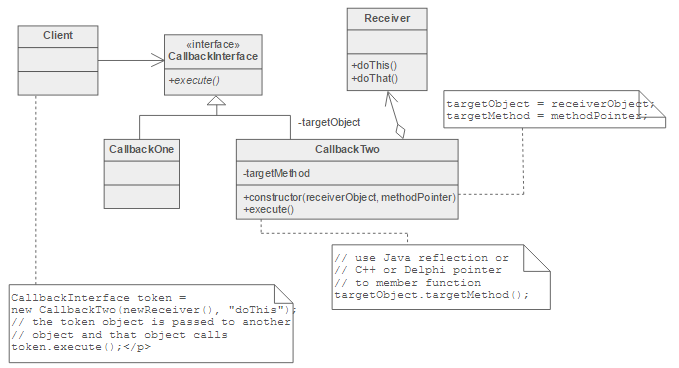
\includegraphics[width=1\linewidth]{images/command.png}
    \caption{Patrón de comportamiento \textit{command}.}\label{diaClases}
\end{figure}


\section{Diagrama de estados}

\begin{figure}[H]
	\centering
    \includegraphics[width=0.4\linewidth]{images/diagEstado.png}
    \caption{Diagrama de estados del procesamiento de un lote.}\label{diaEstado}
\end{figure}

Este diagrama hace referencia de los estados de cada uno de los elementos subidos por el cliente. 

\begin{itemize}
	\item El estado  \textbf {en subida} indica que un lote de imágenes está siendo cargado al sistema y que algunas de las imágenes pueden ya estar almacenadas, pero que no se ha completado el proceso.
    
    \item El estado  \textbf {en proceso} indica que el lote de imágenes está siendo procesado por los algoritmos de preprocesamiento y segmentación, imagen por imagen.
    
    \item El estado  \textbf {interrumpido} indica que un lote de imagen que estaba siendo procesado sufrió una interrupción ya sea de usuario o inesperada, es decir que se encuentra sin terminar.
    
    \item El estado  \textbf {finalizado} indica que un lote de imágenes ha sido completamente procesado y puede ser descargado en su totalidad por el usuario.
    
\end{itemize}



\chapter{Vista de despliegue}

La vista de despliegue ilustra el sistema de la perspectiva del programador y está enfocado en la administración de los artefactos de software. Esta vista también se conoce como vista de implementación. Utiliza el diagrama de componentes UML para describir los componentes de sistema.\\

\section{Diagrama de componentes}

\begin{figure}[H]
	\centering
    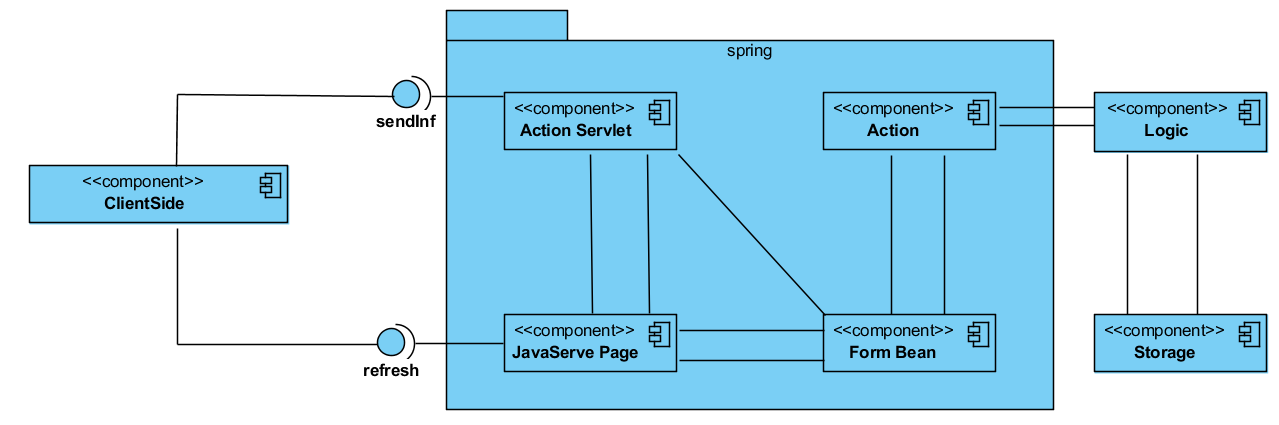
\includegraphics[width=1\linewidth]{images/diagramaComp.png}
    \caption{Diagrama de componentes}
\end{figure}

En el diagrama de componentes se denota la estructura a utilizar, el \textit{framework} de Spring, y la intercomunicación entre sus elementos, mostrando a grandes rasgos el uso de patrones de arquitectura y diseño como MVC y \textit{facade} para la estructura del sistema.

\begin{itemize}
	\item \textit{Client-side:} se actualiza constantemente con el JavaServe Page, mientras que puede enviar peticiones al Action Servlet, que es el encargado de recibir las peticiones. 
	\item \textit{Action Servlet y JavaServe Page:} encargados de las comunicaciones con el cliente. 
    \item \textit{Form bean y Action:} son los elementos intermediarios que determinan las acciones concretas para ejecutar en el área de \textit{logic}. Puede encontrarse una especificación detallada en el diagrama de clases.
    \item \textit{Área logic:} es la encargada de administración y procesos del sistema de datos.
    \item \textit{Storage:} sistemas de bases de datos con las que se comunica el sistema. 
    
\end{itemize}


\chapter{Vista física}

La vista física describe el sistema desde el punto de vista de un ingeniero de sistemas. Está relacionada con la topología de componentes de software en la capa física, así como las conexiones físicas entre estos componentes. En UML, se utiliza el diagrama de despliegue para representar esta vista.\\

\section{Diagrama de despliegue}

\begin{figure}[H]
	\centering
    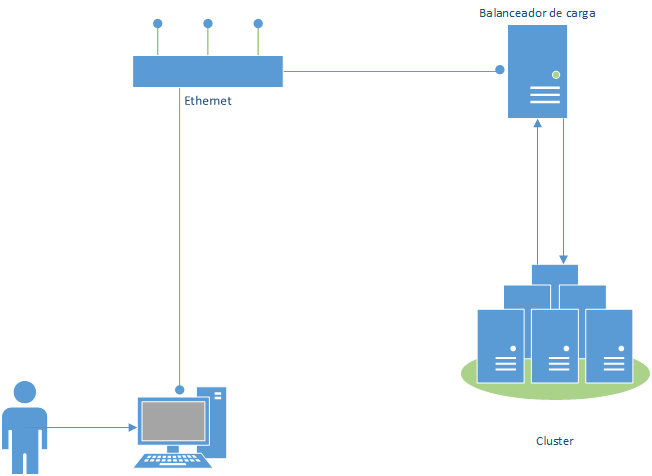
\includegraphics[width=0.75\linewidth]{images/diagDeployment.png}
    \caption{Diagrama de despliegue del sistema.}
\end{figure}

En el diagrama de despliegue muestra un bosquejo de la arquitectura de comunicación del sistema en general. Se le da un enfoque en este diagrama al Ethernet, que representa el enlace de red entre la computadora que usará el usuario y un balanceador de carga que distribuye los trabajos en un clúster. Se propone el uso de una red local, puesto que es más conveniente para el cliente disponer de un complejo computacional potente para correr sus análisis sobre grandes volúmenes de información.


\chapter{Vista de procesos}

La vista de procesos trata los aspectos dinámicos del sistema, explica los procesos de sistema y cómo se comunican. se enfoca en el comportamiento del sistema en tiempo de ejecución. La vista considera aspectos de concurrencia, distribución, rendimiento, escalabilidad, entre otros. En UML se utiliza, por ejemplo, el diagrama de actividad para representar esta vista.\\

\section{Diagrama de actividad}

\begin{figure}[H]
	\centering
    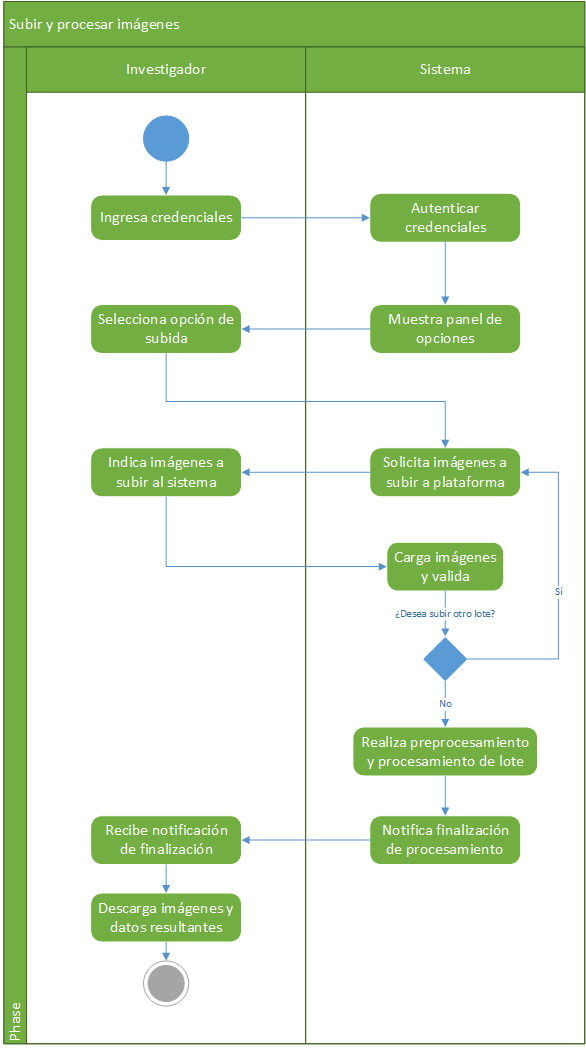
\includegraphics[width=0.5\linewidth]{images/diagActividad.png}
    \caption{Interacción entre el usuario y el sistema.}
\end{figure}

El diagrama de actividad muestra el proceso básico de actividad entre el sistema y el usuario, para exponer los pasos de interacción entre ambos, la funcionalidad del sistema y cómo se comporta cada ente en dicha interacción. Se muestra además el flujo de mensajes entre ambos y las decisiones que puede tomar el usuario "investigador". Este diagrama muestra el flujo básico para que el usuario pueda iniciar el procesamiento de un lote o varios. Se ha mostrado un flujo sencillo que permita la usabilidad como prioridad para el sistema.

\chapter{Vista de escenarios}

La descripción de la arquitectura se ilustra utilizando un conjunto de casos de uso, o escenarios lo que genera una quinta vista. Los escenarios describen secuencias de interacciones entre objetos, y entre procesos. Se utilizan para identificar y validar el diseño de arquitectura. También sirven como punto de partida para pruebas de un prototipo de arquitectura. Esta vista es también conocida como vista de casos de uso.\\

\section{Diagrama de casos de uso}

\begin{figure}[H]
	\centering
    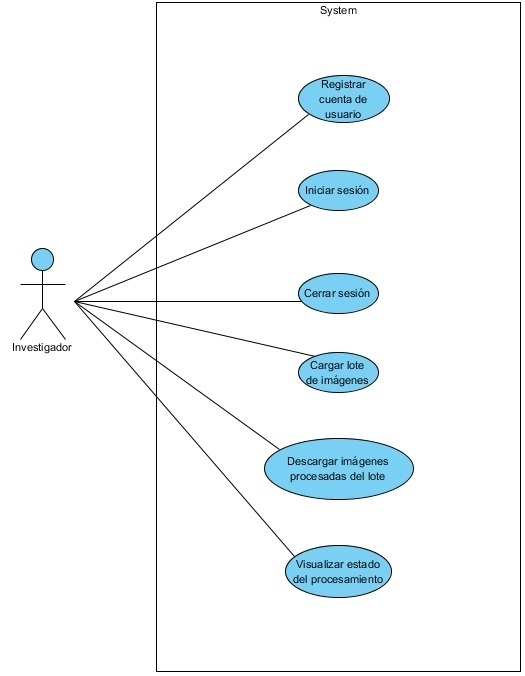
\includegraphics[width=0.7\linewidth]{images/CasosUso.jpg}
    \caption{Diagrama de casos de uso}
\end{figure}



\chapter{Vista adicional: datos}

Esta vista adicional no forma parte del modelo 4 + 1 por definición, pero se ha incluido por su importancia para el sistema. Un modelo de datos permite describir los elementos de la realidad que intervienen en un problema dado y la forma en que se relacionan esos elementos entre sí. En este apartado, se muestra la arquitectura de entidad-relación y el esquema de datos del sistema. Se maneja un modelo tanto relacional como no relacional.\\

\section{Diagrama de Entidad-Relación}
\begin{figure}[H]
	\centering
    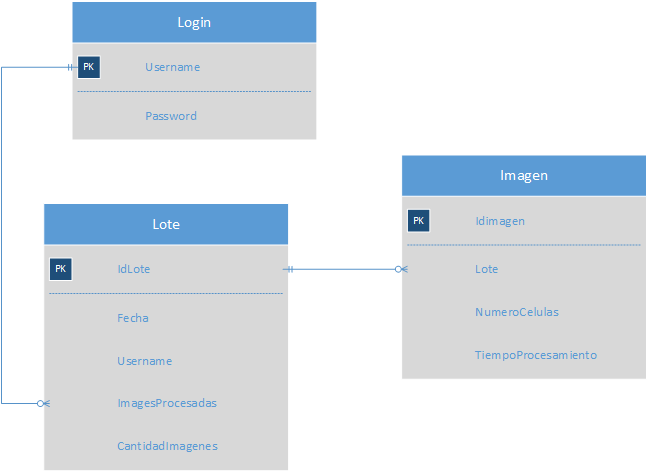
\includegraphics[width=0.7\linewidth]{images/erDiagram.png}
    \caption{Diagrama de Entidad-Relación}
\end{figure}
El diagrama de entidad relación mostrado muestra la estructura de la base de datos relacional que va a tener el sistema. 
Para el manejo de sesiones se tiene la tabla login, que contiene un Username y el password, los cuales permiten el acceso a cada uno de los clientes registrados.
El lote es la representación conceptual de un conjunto de imágenes, los cuales se hacen en un pedido del usuario. Los mismos tienen una fecha de inicio y además un contador que permite verificar cuánto es el monto de imagenes relacionados a cada uno de ellos.\\

Es importante añadir que la tabla "imagenes" en la base de datos relacional contiene por cada tupla un identificador, un numero de células (dato que se actualiza cuando la imagen fue procesada) y el tiempo transcurrido por imagen. \\

Nota: no se almacenarán en ningún momento del proceso las imágenes en la base de datos relacional, puesto que se tiene las base de datos NoSQL dedicadas al almacenamiento de las imágenes obtenidas.

\section{Esquema de datos (NoSQL)}

\begin{figure}[H]
	\centering
    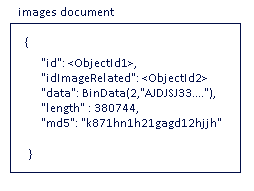
\includegraphics[width=0.5\linewidth]{images/mongo.png}
    \caption{Esquema de datos (mongodb)}
\end{figure}

El esquema de datos es una representación de la base de datos no relacional, mongodb. La cual se va a utilizar para el almacenamiento de las imagenes en el sistema. En el diagrama se muestra las propiedades que contiene este:

\begin{itemize}
	\item \textit{Id:} es un identificador que tiene cada elemento dentro de la base de datos.
    \item \textit{IdImageRelated:} es un identificador que esta asociado a un elemento en la base de datos relacional.
    \item \textit{Data:} Almacena en dato binario la imagen obtenida del usuario.
    \item \textit{Lenght:} determina el largo del archivo recibido, como medida de seguridad.
    \item \textit{Md5:} es el cifrado de la imagen en formato Md5.
    
\end{itemize}


\end{document}